As shown in Table~\ref{tab:bench} and Figures~\ref{fig:states}--\ref{fig:memory}, A* typically explores far fewer states and avoids timeouts where BFS fails.

\begin{figure}[H] 
\centering
\begin{minipage}{0.48\textwidth}
    \centering
    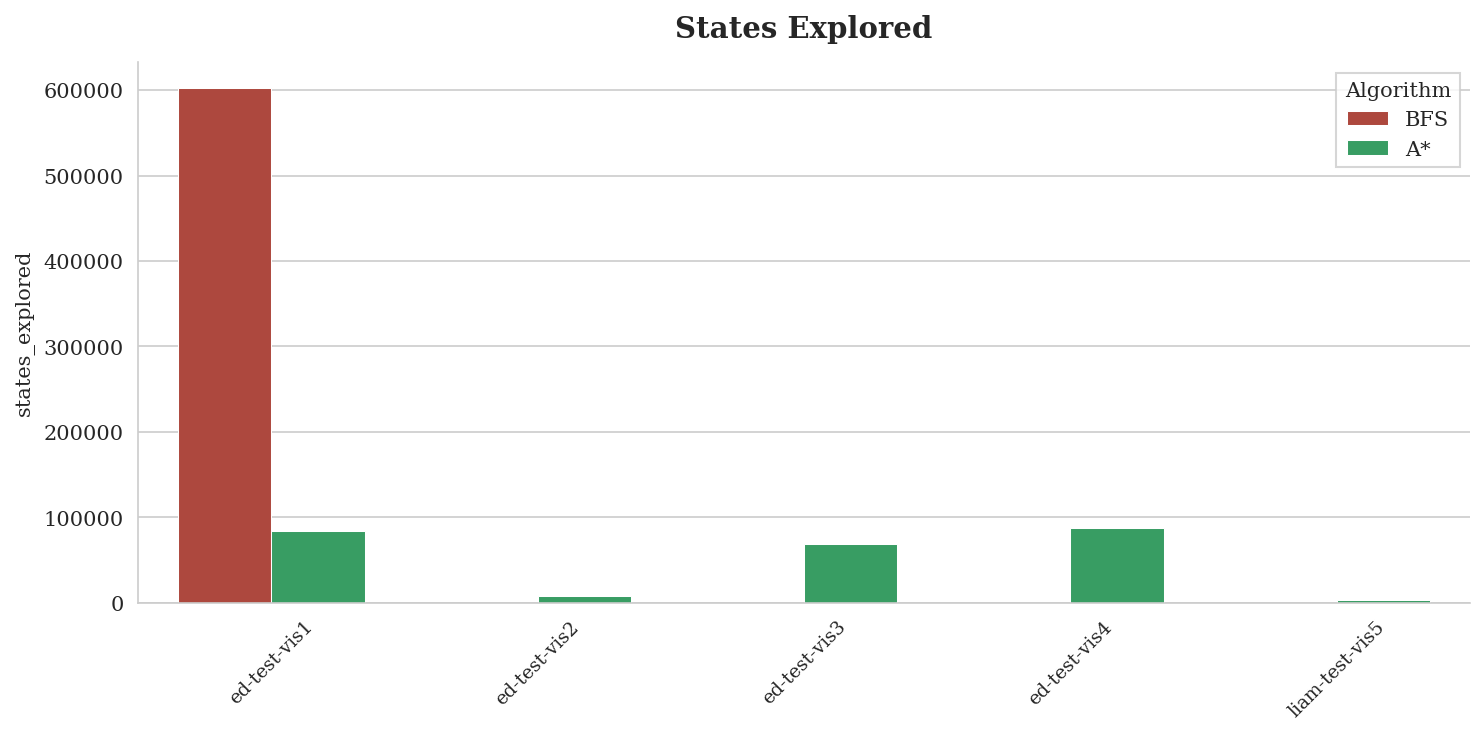
\includegraphics[width=\linewidth]{benchmark_states.png}
    \caption{States}\label{fig:states}
\end{minipage}\hfill
\begin{minipage}{0.48\textwidth}
    \centering
    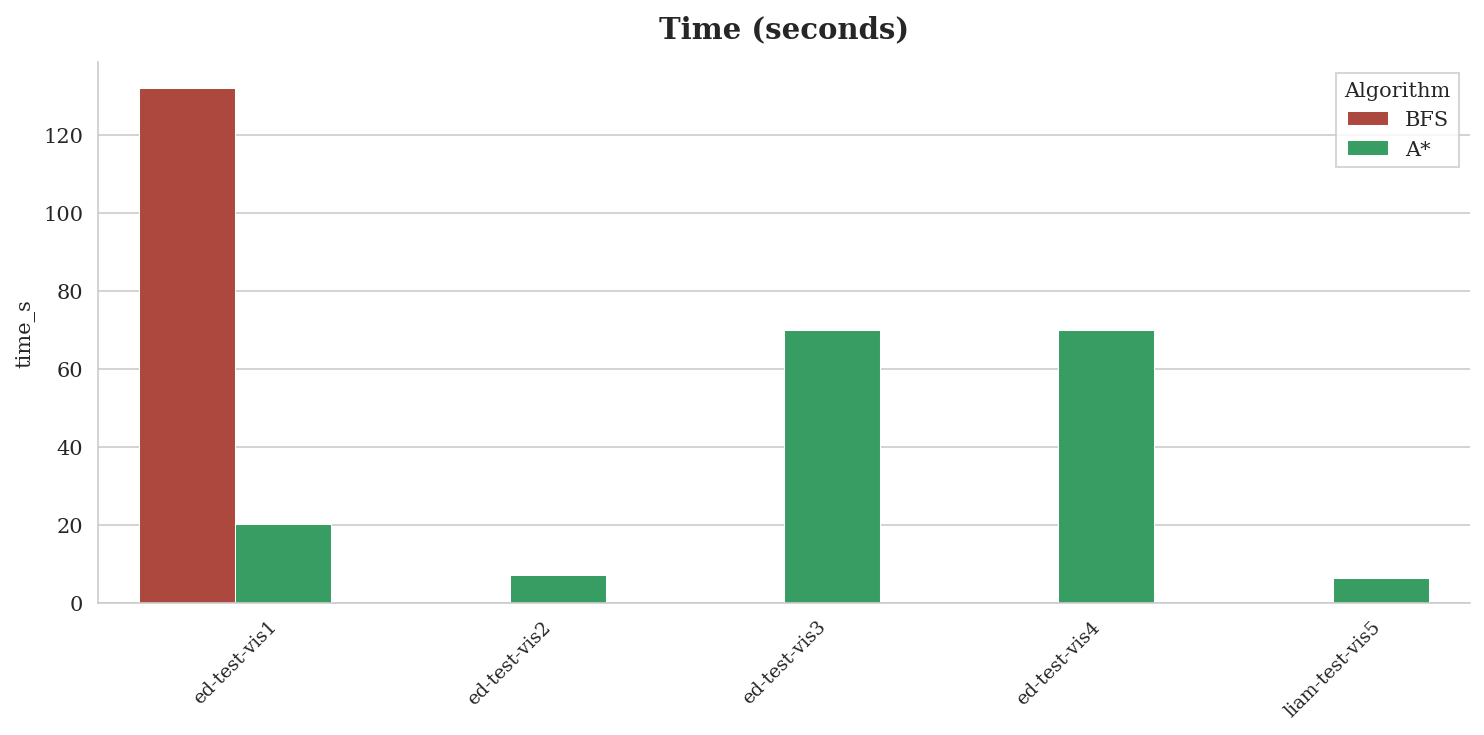
\includegraphics[width=\linewidth]{benchmark_time.png}
    \caption{Time (s)}\label{fig:time}
\end{minipage}

\vspace{1.5em} 

\begin{minipage}{0.5\textwidth}
    \centering
    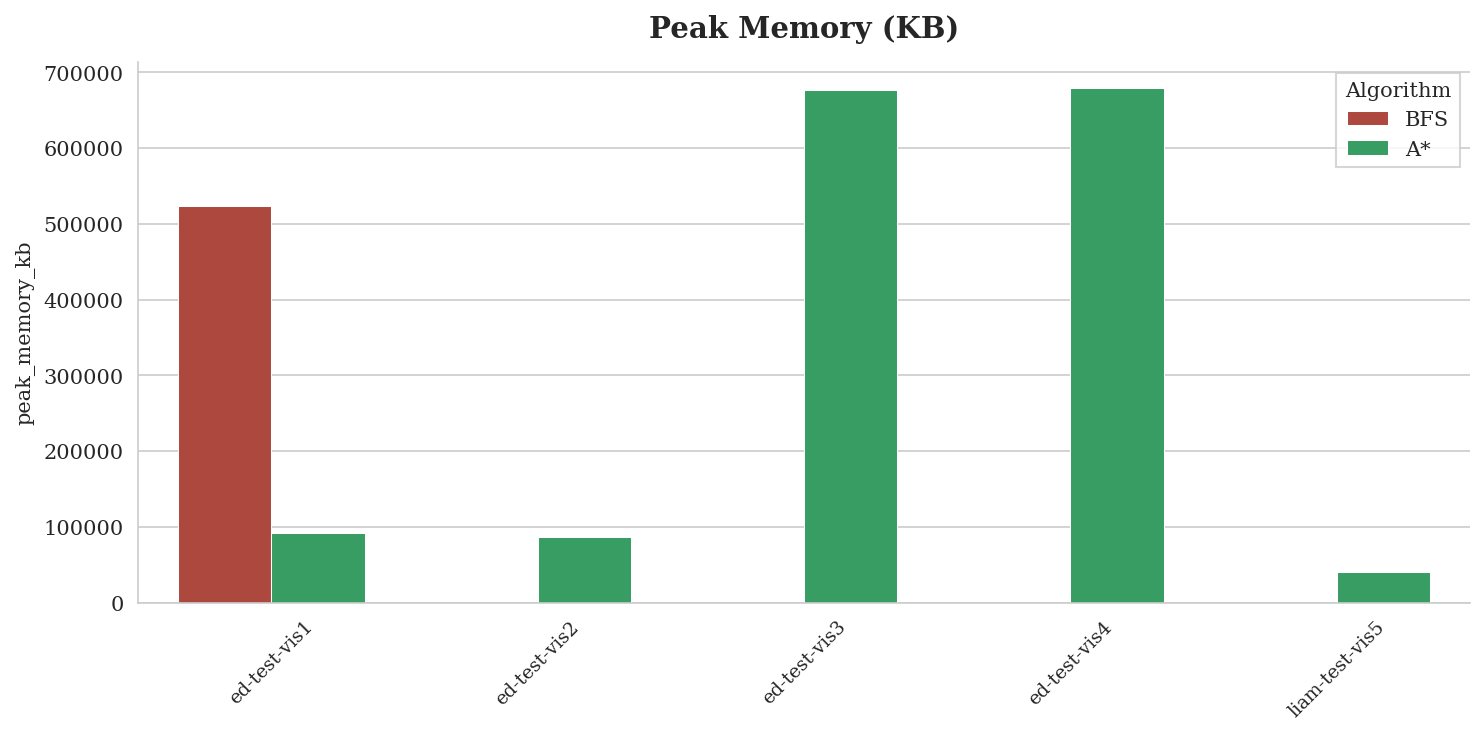
\includegraphics[width=\linewidth]{benchmark_memory.png}
    \caption{Memory (KB)}\label{fig:memory}
\end{minipage}
\end{figure}